\tikzset{every picture/.style={line width=0.75pt}} %set default line width to 0.75pt        

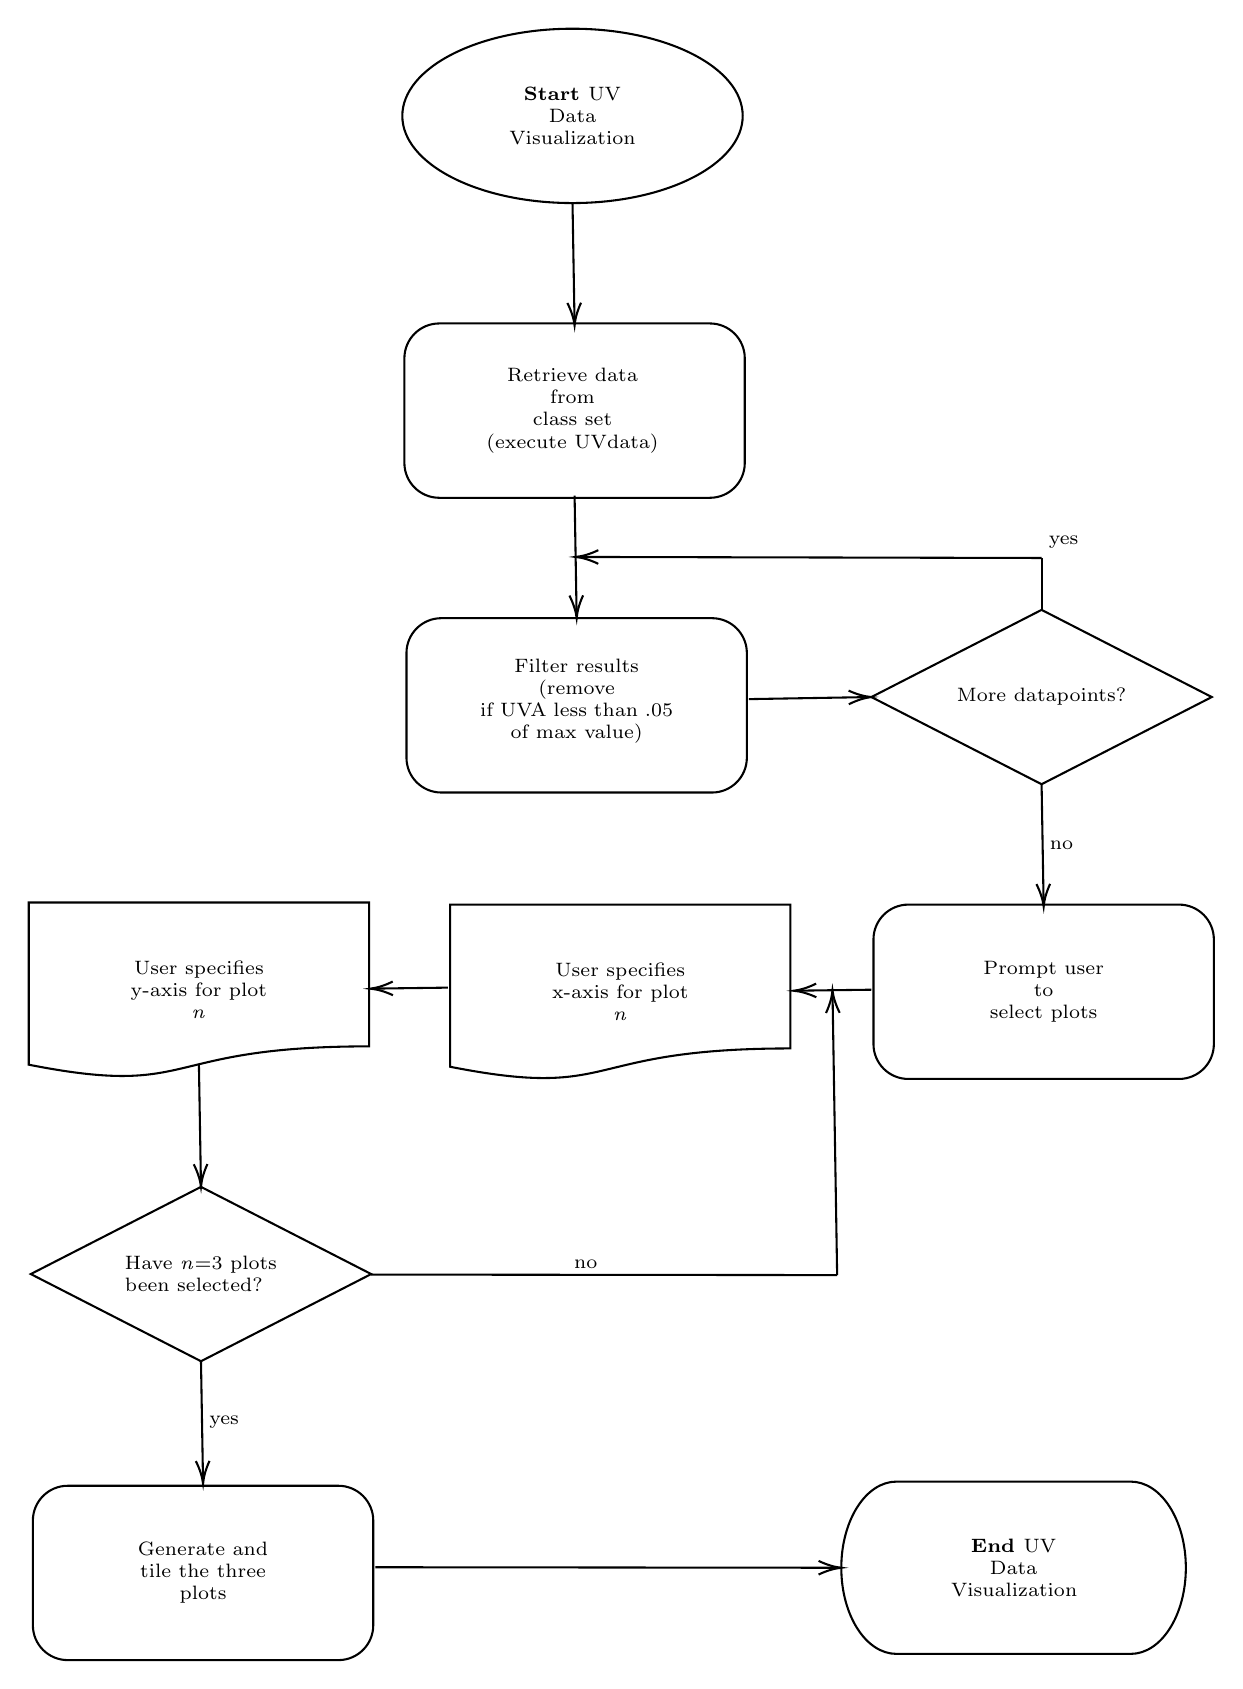
\begin{tikzpicture}[x=0.75pt,y=0.75pt,yscale=-1,xscale=1]
%uncomment if require: \path (0,792); %set diagram left start at 0, and has height of 792

%Shape: Ellipse [id:dp25065506264197857] 
\draw   (207,45) .. controls (207,21.8) and (243.71,3) .. (289,3) .. controls (334.29,3) and (371,21.8) .. (371,45) .. controls (371,68.2) and (334.29,87) .. (289,87) .. controls (243.71,87) and (207,68.2) .. (207,45) -- cycle ;
%Straight Lines [id:da7860264738763125] 
\draw    (289,87) -- (289.97,144) ;
\draw [shift={(290,146)}, rotate = 269.03] [color={rgb, 255:red, 0; green, 0; blue, 0 }  ][line width=0.75]    (10.93,-3.29) .. controls (6.95,-1.4) and (3.31,-0.3) .. (0,0) .. controls (3.31,0.3) and (6.95,1.4) .. (10.93,3.29)   ;
%Rounded Rect [id:dp38520792496580514] 
\draw   (208,161.8) .. controls (208,152.52) and (215.52,145) .. (224.8,145) -- (355.2,145) .. controls (364.48,145) and (372,152.52) .. (372,161.8) -- (372,212.2) .. controls (372,221.48) and (364.48,229) .. (355.2,229) -- (224.8,229) .. controls (215.52,229) and (208,221.48) .. (208,212.2) -- cycle ;
%Straight Lines [id:da12554765645866106] 
\draw    (290,228) -- (290.97,285) ;
\draw [shift={(291,287)}, rotate = 269.03] [color={rgb, 255:red, 0; green, 0; blue, 0 }  ][line width=0.75]    (10.93,-3.29) .. controls (6.95,-1.4) and (3.31,-0.3) .. (0,0) .. controls (3.31,0.3) and (6.95,1.4) .. (10.93,3.29)   ;
%Rounded Rect [id:dp8809468446489852] 
\draw   (209,303.8) .. controls (209,294.52) and (216.52,287) .. (225.8,287) -- (356.2,287) .. controls (365.48,287) and (373,294.52) .. (373,303.8) -- (373,354.2) .. controls (373,363.48) and (365.48,371) .. (356.2,371) -- (225.8,371) .. controls (216.52,371) and (209,363.48) .. (209,354.2) -- cycle ;
%Flowchart: Decision [id:dp33612075100452476] 
\draw   (515,283) -- (597,325) -- (515,367) -- (433,325) -- cycle ;
%Shape: Boxed Line [id:dp9856035467294029] 
\draw    (374,326) -- (431,325.03) ;
\draw [shift={(433,325)}, rotate = 179.03] [color={rgb, 255:red, 0; green, 0; blue, 0 }  ][line width=0.75]    (10.93,-3.29) .. controls (6.95,-1.4) and (3.31,-0.3) .. (0,0) .. controls (3.31,0.3) and (6.95,1.4) .. (10.93,3.29)   ;
%Straight Lines [id:da09631140250278603] 
\draw    (515,258) -- (515,283) ;
%Straight Lines [id:da9736702197505198] 
\draw    (515,258) -- (292.5,257.5) ;
\draw [shift={(290.5,257.5)}, rotate = 0.13] [color={rgb, 255:red, 0; green, 0; blue, 0 }  ][line width=0.75]    (10.93,-3.29) .. controls (6.95,-1.4) and (3.31,-0.3) .. (0,0) .. controls (3.31,0.3) and (6.95,1.4) .. (10.93,3.29)   ;
%Rounded Rect [id:dp6172850573909681] 
\draw   (434,441.8) .. controls (434,432.52) and (441.52,425) .. (450.8,425) -- (581.2,425) .. controls (590.48,425) and (598,432.52) .. (598,441.8) -- (598,492.2) .. controls (598,501.48) and (590.48,509) .. (581.2,509) -- (450.8,509) .. controls (441.52,509) and (434,501.48) .. (434,492.2) -- cycle ;
%Straight Lines [id:da024983221440428638] 
\draw    (515,367) -- (515.97,424) ;
\draw [shift={(516,426)}, rotate = 269.03] [color={rgb, 255:red, 0; green, 0; blue, 0 }  ][line width=0.75]    (10.93,-3.29) .. controls (6.95,-1.4) and (3.31,-0.3) .. (0,0) .. controls (3.31,0.3) and (6.95,1.4) .. (10.93,3.29)   ;
%Flowchart: Document [id:dp3943133798804599] 
\draw   (230,425) -- (394,425) -- (394,494.3) .. controls (291.5,494.3) and (312,519.29) .. (230,503.12) -- cycle ;
%Straight Lines [id:da6781395973359248] 
\draw    (229,465) -- (193.5,465.47) ;
\draw [shift={(191.5,465.5)}, rotate = 359.24] [color={rgb, 255:red, 0; green, 0; blue, 0 }  ][line width=0.75]    (10.93,-3.29) .. controls (6.95,-1.4) and (3.31,-0.3) .. (0,0) .. controls (3.31,0.3) and (6.95,1.4) .. (10.93,3.29)   ;
%Flowchart: Document [id:dp3217398265719609] 
\draw   (27,424) -- (191,424) -- (191,493.3) .. controls (88.5,493.3) and (109,518.29) .. (27,502.12) -- cycle ;
%Straight Lines [id:da5463827574200826] 
\draw    (433,466) -- (397.5,466.47) ;
\draw [shift={(395.5,466.5)}, rotate = 359.24] [color={rgb, 255:red, 0; green, 0; blue, 0 }  ][line width=0.75]    (10.93,-3.29) .. controls (6.95,-1.4) and (3.31,-0.3) .. (0,0) .. controls (3.31,0.3) and (6.95,1.4) .. (10.93,3.29)   ;
%Straight Lines [id:da5254918143426153] 
\draw    (109,502) -- (109.97,559) ;
\draw [shift={(110,561)}, rotate = 269.03] [color={rgb, 255:red, 0; green, 0; blue, 0 }  ][line width=0.75]    (10.93,-3.29) .. controls (6.95,-1.4) and (3.31,-0.3) .. (0,0) .. controls (3.31,0.3) and (6.95,1.4) .. (10.93,3.29)   ;
%Flowchart: Decision [id:dp6448891128840071] 
\draw   (110,561) -- (192,603) -- (110,645) -- (28,603) -- cycle ;
%Straight Lines [id:da9240837376905715] 
\draw    (192,603.25) -- (416.5,603.5) ;
%Straight Lines [id:da5905876865001083] 
\draw    (416.5,603.5) -- (414.28,468.25) ;
\draw [shift={(414.25,466.25)}, rotate = 89.06] [color={rgb, 255:red, 0; green, 0; blue, 0 }  ][line width=0.75]    (10.93,-3.29) .. controls (6.95,-1.4) and (3.31,-0.3) .. (0,0) .. controls (3.31,0.3) and (6.95,1.4) .. (10.93,3.29)   ;
%Straight Lines [id:da2900668037368952] 
\draw    (110,645) -- (110.97,702) ;
\draw [shift={(111,704)}, rotate = 269.03] [color={rgb, 255:red, 0; green, 0; blue, 0 }  ][line width=0.75]    (10.93,-3.29) .. controls (6.95,-1.4) and (3.31,-0.3) .. (0,0) .. controls (3.31,0.3) and (6.95,1.4) .. (10.93,3.29)   ;
%Rounded Rect [id:dp5291972841653532] 
\draw   (29,721.8) .. controls (29,712.52) and (36.52,705) .. (45.8,705) -- (176.2,705) .. controls (185.48,705) and (193,712.52) .. (193,721.8) -- (193,772.2) .. controls (193,781.48) and (185.48,789) .. (176.2,789) -- (45.8,789) .. controls (36.52,789) and (29,781.48) .. (29,772.2) -- cycle ;
%Straight Lines [id:da1281453542926556] 
\draw    (194,744.25) -- (416.5,744.5) ;
\draw [shift={(418.5,744.5)}, rotate = 180.06] [color={rgb, 255:red, 0; green, 0; blue, 0 }  ][line width=0.75]    (10.93,-3.29) .. controls (6.95,-1.4) and (3.31,-0.3) .. (0,0) .. controls (3.31,0.3) and (6.95,1.4) .. (10.93,3.29)   ;
%Flowchart: Terminator [id:dp3943034545708537] 
\draw   (445.06,703) -- (557.94,703) .. controls (572.61,703) and (584.5,721.58) .. (584.5,744.5) .. controls (584.5,767.42) and (572.61,786) .. (557.94,786) -- (445.06,786) .. controls (430.39,786) and (418.5,767.42) .. (418.5,744.5) .. controls (418.5,721.58) and (430.39,703) .. (445.06,703) -- cycle ;

% Text Node
\draw (289,45) node  [font=\scriptsize] [align=left] {\begin{minipage}[lt]{47.96pt}\setlength\topsep{0pt}
\begin{center}
\textbf{Start }UV Data\\Visualization
\end{center}

\end{minipage}};
% Text Node
\draw (289,187) node  [font=\scriptsize] [align=left] {\begin{minipage}[lt]{63.44pt}\setlength\topsep{0pt}
\begin{center}
Retrieve data from \\class set \\(execute UVdata)
\end{center}

\end{minipage}};
% Text Node
\draw (291,327) node  [font=\scriptsize] [align=left] {\begin{minipage}[lt]{69.77pt}\setlength\topsep{0pt}
\begin{center}
Filter results (remove\\if UVA less than .05\\of max value)
\end{center}

\end{minipage}};
% Text Node
\draw (515,325) node  [font=\scriptsize] [align=left] {More datapoints?};
% Text Node
\draw (517,255) node [anchor=south west] [inner sep=0.75pt]  [font=\scriptsize] [align=left] {yes};
% Text Node
\draw (517.5,396.5) node [anchor=west] [inner sep=0.75pt]  [font=\scriptsize] [align=left] {no};
% Text Node
\draw (516,467) node  [font=\scriptsize] [align=left] {\begin{minipage}[lt]{49.56pt}\setlength\topsep{0pt}
\begin{center}
Prompt user to\\select plots
\end{center}

\end{minipage}};
% Text Node
\draw (312,467) node  [font=\scriptsize] [align=left] {\begin{minipage}[lt]{51.14pt}\setlength\topsep{0pt}
\begin{center}
User specifies\\x-axis for plot \textit{n}
\end{center}

\end{minipage}};
% Text Node
\draw (109,466) node  [font=\scriptsize] [align=left] {\begin{minipage}[lt]{51.14pt}\setlength\topsep{0pt}
\begin{center}
User specifies\\y-axis for plot \textit{n}
\end{center}

\end{minipage}};
% Text Node
\draw (110,603) node  [font=\scriptsize] [align=left] {Have \textit{n}=3 plots\\been selected?};
% Text Node
\draw (295.34,602) node [anchor=south] [inner sep=0.75pt]  [font=\scriptsize] [align=left] {no};
% Text Node
\draw (112.5,674.5) node [anchor=west] [inner sep=0.75pt]  [font=\scriptsize] [align=left] {yes};
% Text Node
\draw (111,747) node  [font=\scriptsize] [align=left] {\begin{minipage}[lt]{59.09pt}\setlength\topsep{0pt}
\begin{center}
Generate and\\tile the three plots
\end{center}

\end{minipage}};
% Text Node
\draw (501.5,744.5) node  [font=\scriptsize] [align=left] {\begin{minipage}[lt]{45.18pt}\setlength\topsep{0pt}
\begin{center}
\textbf{End }UV Data\\Visualization
\end{center}

\end{minipage}};


\end{tikzpicture}
